\section{Signals and Readout}

There are 512 channels per module read out by FSSR2 chips, mounted on a hybrid. The FSSR2 ASIC has been developed at Fermilab for the BTeV experiment \cite{FSSR}. The chip (see Fig.~\ref{fig:fssr2}) features a data-driven architecture (self-triggered, time-stamped). Each of the 128 input channels of the FSSR2 ASIC has a preamplifier, a shaper that can adjust the shaping time (50--125~ns), a baseline restorer (BLR), and a 3-bit ADC (see Fig.~\ref{fig:fssr2-analog}). The period of the clock called the beam crossing oscillator (BCO) sets the data acquisition time. 

\begin{figure}[hbt] 
\centering 
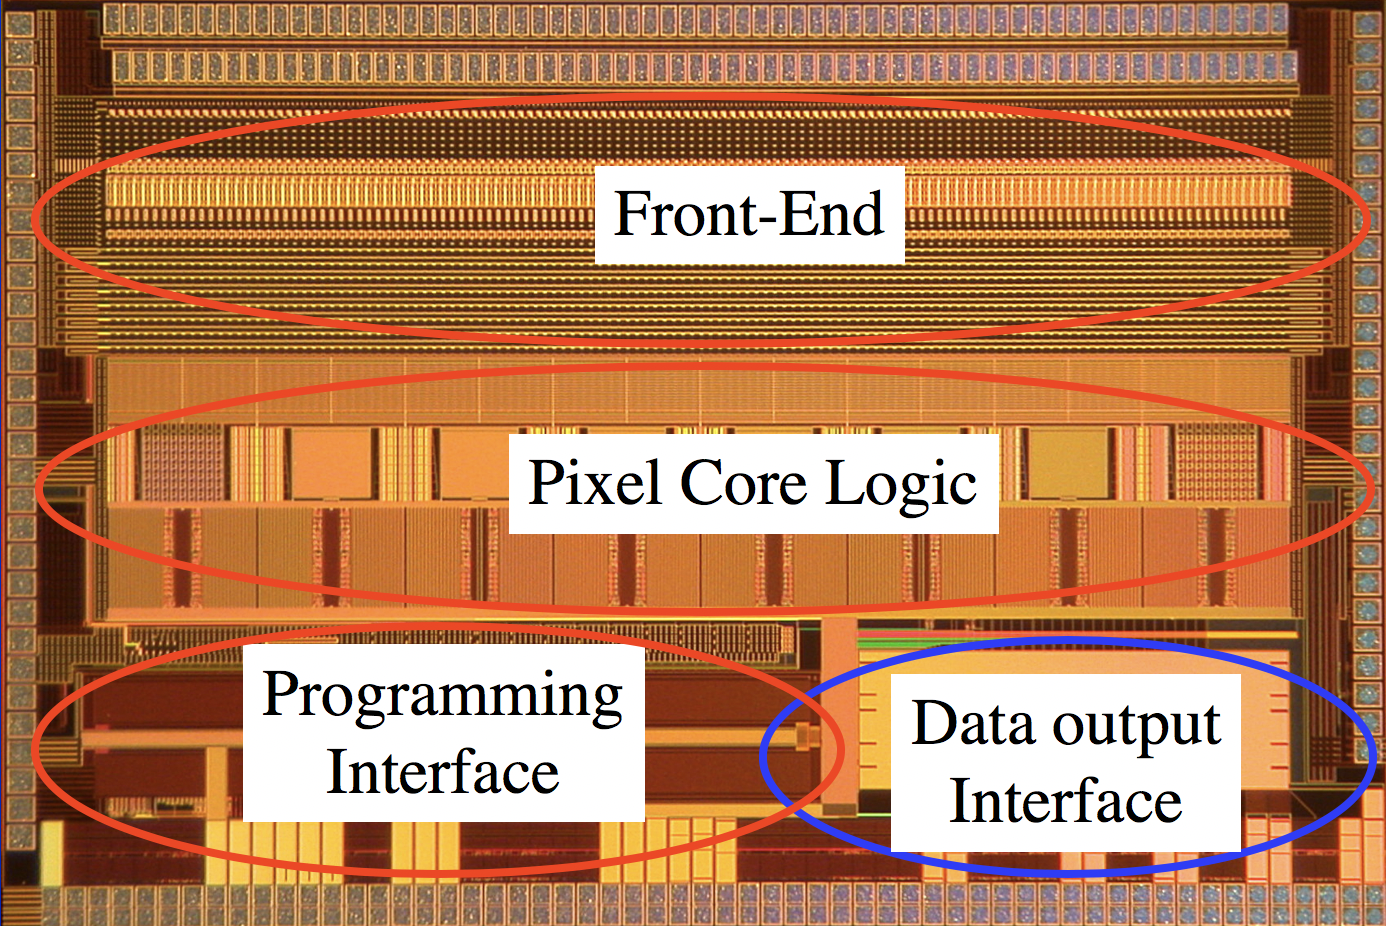
\includegraphics[width=0.8\columnwidth,keepaspectratio]{fssr2.png}
\caption{FSSR2 ASIC with the different functional areas labeled.}
\label{fig:fssr2}
\end{figure}

\begin{figure}[hbt] 
\centering 
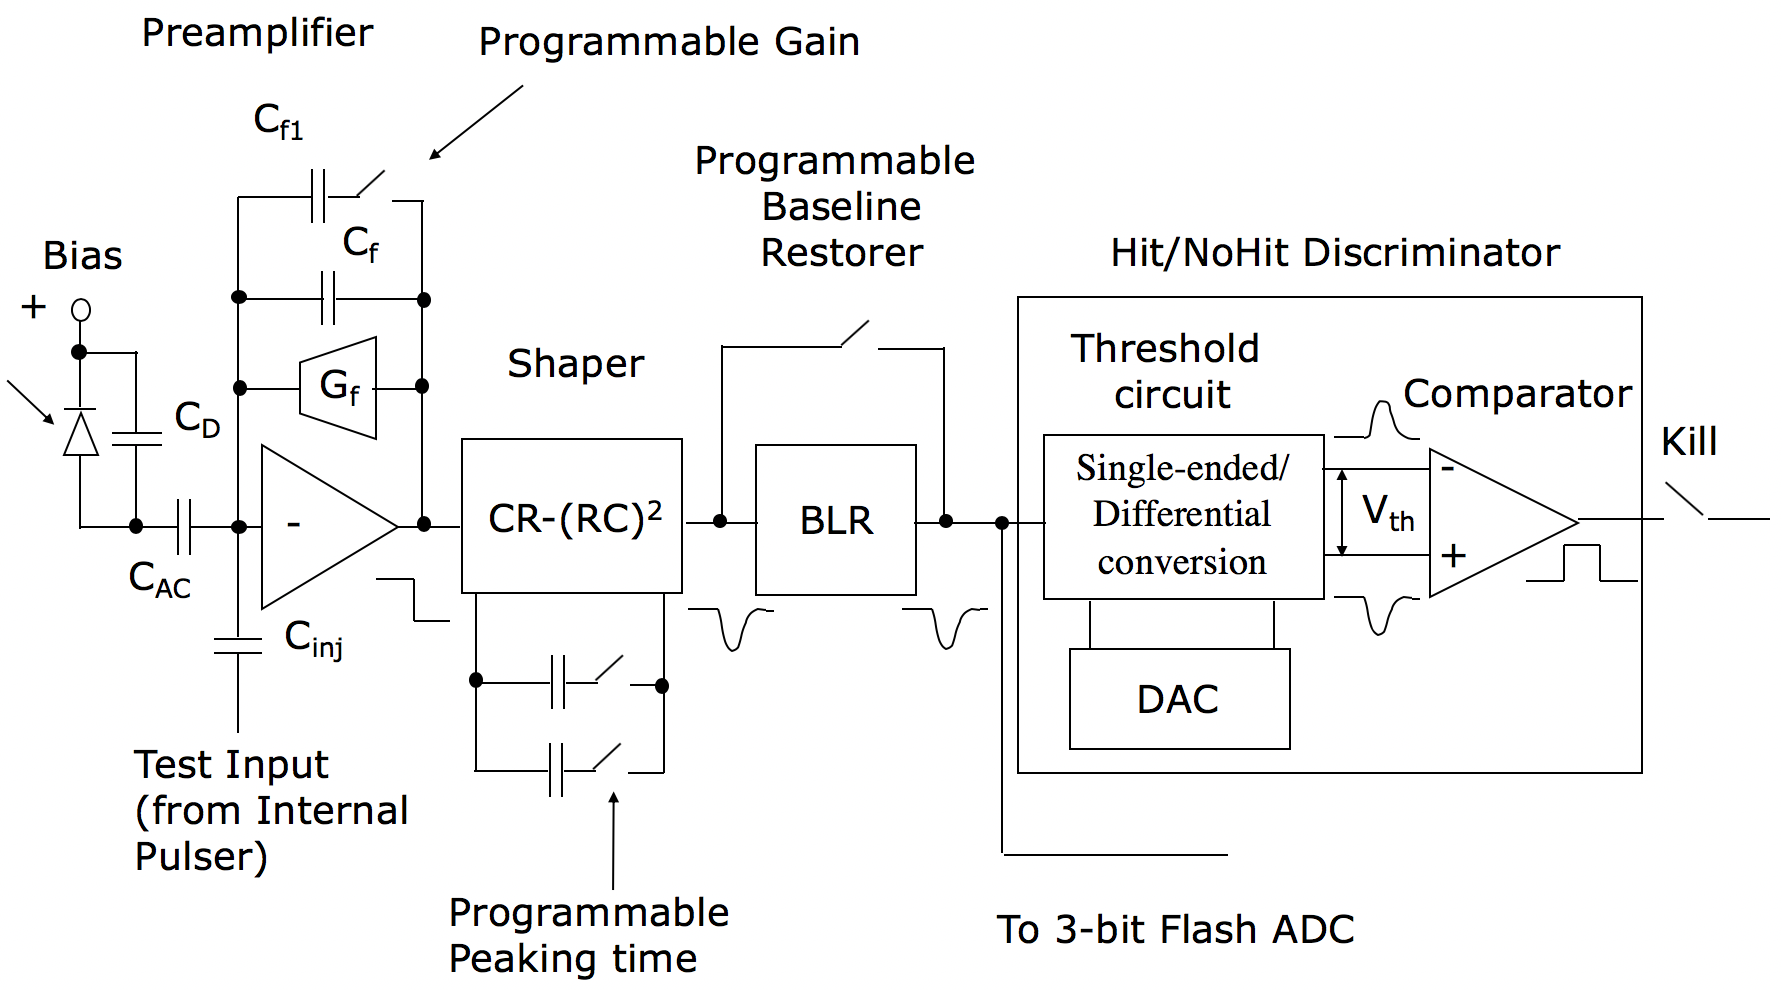
\includegraphics[width=1.0\columnwidth,keepaspectratio]{fssr2-analog.png}
\caption{FSSR2 analog channels.}
\label{fig:fssr2-analog}
\end{figure}

If a hit is detected in one of the channels, the core logic transmits pulse amplitude, channel number, and time stamp information to the data output interface. The data output interface accepts data transmitted by the core, serializes it, and transmits it to the data acquisition system. To send the 24-bit readout words one, two, four, or six LVDS serial data lines can be used. Both edges of the 70~MHz readout clock are used to clock data, resulting in a maximum output data rate of 840 Mb/s. The readout clock is independent of the acquisition clock. Power consumption is $\le$ 4~mW per channel. The FSSR2 is radiation hard up to 5~Mrad. The choice of the readout chip was driven by its architecture and good noise performance (see Fig.~\ref{fig:fssr2-enc-c}) at high capacitive load of long SVT strips.

\begin{figure}[hbt] 
\centering 
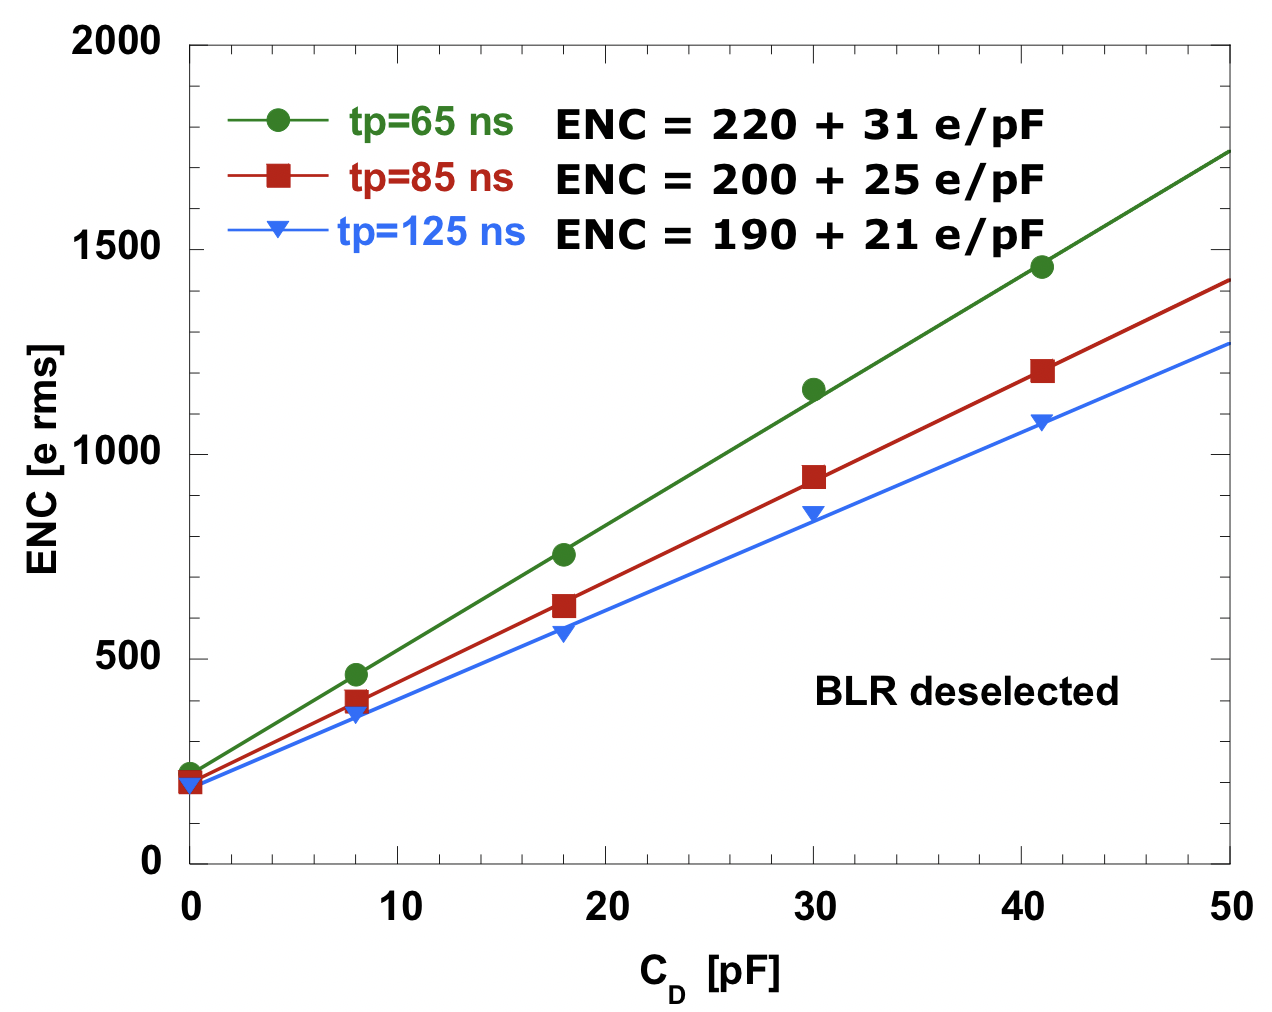
\includegraphics[width=1.0\columnwidth,keepaspectratio]{fssr2-enc-c.png}
\caption{FSSR2 equivalent noise charge vs. detector capacitance at different shaping time settings.}
\label{fig:fssr2-enc-c}
\end{figure}

The four FSSR2 ASICs on the HFCB communicate with the VXS architecture-based segment collector module (VSCM), which configures the FSSR2 ASIC registers, provides analog calibration pulses to the FSSR2 ASICs, sets/monitors proper control signals (clock, reset, status), and acquires serialized event data from the FSSR2 ASICs. Each VSCM can interface with two HFCBs. Up to 16 VSCM cards can reside in a VXS crate. When multiple VSCM cards are used, additional cards, the Trigger Interface (TI), and Signal Distribution (SD), are required to ensure event and timing synchronization. The VSCM supports a stand-alone mode, useful when only one or two HFCBs are used. 

Each FSSR2 ASICs has six LVDS pairs with a source synchronous clock to transmit event data. The VSCM supports receiving data from all six LVDS pairs of each FSSR2 ASIC running at 70 MHz double data rate (DDR) (840 Mb/s from each FSSR2). Xilinx Spartan 6 FPGAs are used to buffer and deserialize data from two FSSR2 ASICs each. Four of these FPGAs are used to support eight FSSR2 ASICs' simultaneous data streams coming from two HFCB interfaces; the FPGAs in turn send their information to the master FPGA where the event builder resides.

The FSSR2 ASICs' architecture is such that it sends out 24-bit data words if a channel has a hit or a 24-bit status word if the channel does not have a hit (idle state) within a BCO clock cycle. The FSSR2 ASICs transmit these data over six lines. First, the data is de-serialized. The 24-bit data words are appended with 8 bits to make the time range longer, and the 32-bit words are correlated to the trigger, which is generated by other detectors. The status words are suppressed to minimize the data size of an event. However, the status words are monitored to diagnose the performance of individual FSSR2 ASICs. The event builder of the VSCM uses the BCO clock timestamp from the data word of each FSSR2 ASIC and matches it to the timestamp of the global system clock, given by the CLAS12 trigger. The FSSR2 ASIC data is tagged with a global trigger timestamp (48 bits, 8 ns resolution). Since the BCO clock is derived from the global system clock, triggers received by the VSCM enable the event builder to extract hits with specific BCO timestamps that fall in a programmable time window within which the event could have occurred. When a trigger is received, the data words from the FSSR2 ASICs are copied to an event buffer and pushed into an event FIFO. These events can be read out in order with other modules in the system while event-level synchronization across all modules in the system is maintained. The VME interface provides for event readout, access to the configuration registers on the VSCM, bridges access to the registers of the FSSR2 ASICs, and provides an interface to the CPU. The A32 address space, 2 MB in size, is dedicated to the event builder FIFO, which can be read using single-cycle and block transfer VME protocols. Block transfer protocols are used for event readout; the 2eSST protocol planned for use is to maximize performance. The 2eSST protocols provide ~200 MB/s sustained transfer rate and supports the proprietary Jefferson Lab token-passing scheme that allows a single direct memory access (DMA) operation on the CPU to transfer data from all VSCM modules sequentially, eliminating overhead (compared to individual board transfers). The VSCM is set up to extract event data within a programmable lookback window of $\sim$16~$\mu$s relative to the received trigger. 

The calibration pulser circuit provides a 2 Vpp dynamic range, up to 125 MS/s, and 14-bit resolution (for pulse height steps in sub mV increments). The bandwidth is sufficient to allow 10 ns rise times to be delivered over 15 feet of 50~$\Omega$ coax cable terminated with 50~$\Omega$. Two independent pulser outputs are provided to drive both HFCB modules. The pulser signal phase can be placed in a deterministic phase relationship to the BCO clock that drives the FSSR2 ASIC.
